% Source PDF page 171 (printed p. 157)
\subsubsection*{鲁棒线性规划}
考虑不等式形式的线性规划
\[
\begin{array}{ll}\text{最小化}&c^\T x\\\text{约束为}&a_i^\T x\le b_i,\quad i=1,\ldots,m,\end{array}
\]
其中参数 $c,a_i,b_i$ 存在不确定性或变化。为简化叙述，假设 $c,b_i$ 固定，而已知 $a_i$ 位于给定椭球中：
\[
a_i\in\mathcal E_i=\{\bar a_i+P_iu\mid\norm{u}_2\le1\},
\]
其中 $P_i\in\R^{n\times n}$。（若 $P_i$ 奇异，得到维数为 $\rank P_i$ 的“扁平”椭球；$P_i=0$ 表示完全知道 $a_i$。）

我们要求对参数 $a_i$ 的所有可能取值，约束都成立，由此得到鲁棒线性规划
\begin{equation}
\begin{array}{ll}\text{最小化}&c^\T x\\\text{约束为}&a_i^\T x\le b_i\quad\text{对所有 }a_i\in\mathcal E_i,\quad i=1,\ldots,m.\end{array}\tag{4.37}
\end{equation}
鲁棒线性约束“对所有 $a_i\in\mathcal E_i$，有 $a_i^\T x\le b_i$”可写为
\[
\sup\{a_i^\T x\mid a_i\in\mathcal E_i\}\le b_i,
\]
其左侧为
\[
\begin{aligned}
\sup\{a_i^\T x\mid a_i\in\mathcal E_i\}
&=\bar a_i^\T x+\sup\{u^\T P_i^\T x\mid\norm{u}_2\le1\}\\
&=\bar a_i^\T x+\norm{P_i^\T x}_2.
\end{aligned}
\]
因此，鲁棒线性约束可以表示为
\[
\bar a_i^\T x+\norm{P_i^\T x}_2\le b_i,
\]
它显然是二阶锥约束。所以鲁棒LP（4.37）可表示为SOCP
\[
\begin{array}{ll}\text{最小化}&c^\T x\\\text{约束为}&\bar a_i^\T x+\norm{P_i^\T x}_2\le b_i,\quad i=1,\ldots,m.\end{array}
\]
注意，增加的范数项起着正则化作用；它们防止 $x$ 在参数 $a_i$ 不确定性较大的方向上取得过大的值。

\subsubsection*{带随机约束的线性规划}
上述鲁棒LP也可以在统计框架下考虑。假设参数 $a_i$ 是相互独立的高斯随机向量，均值为 $\bar a_i$、协方差为 $\Sigma_i$。要求每个约束 $a_i^\T x\le b_i$ 成立的概率或置信度超过 $\eta$，其中 $\eta\ge0.5$，即
\begin{equation}
\Prob(a_i^\T x\le b_i)\ge\eta.\tag{4.38}
\end{equation}

% Source PDF page 172 (printed p. 158)
我们将说明这个概率约束可表示为二阶锥约束。

令 $u=a_i^\T x$，以 $\sigma^2$ 表示其方差，则约束可写为
\[
\Prob\left(\frac{u-\bar u}{\sigma}\le\frac{b_i-\bar u}{\sigma}\right)\ge\eta.
\]
由于 $(u-\bar u)/\sigma$ 是零均值、单位方差的高斯变量，上述概率就是 $\Phi((b_i-\bar u)/\sigma)$，其中
\[
\Phi(z)=\frac1{\sqrt{2\pi}}\int_{-\infty}^z e^{-t^2/2}\,dt
\]
是零均值、单位方差高斯随机变量的累积分布函数。因此，概率约束（4.38）可表示为
\[
\frac{b_i-\bar u}{\sigma}\ge\Phi^{-1}(\eta),
\]
或等价地
\[
\bar u+\Phi^{-1}(\eta)\sigma\le b_i.
\]
利用 $\bar u=\bar a_i^\T x$、$\sigma=(x^\T\Sigma_i x)^{1/2}$，得到
\[
\bar a_i^\T x+\Phi^{-1}(\eta)\norm{\Sigma_i^{1/2}x}_2\le b_i.
\]
根据假设 $\eta\ge1/2$，有 $\Phi^{-1}(\eta)\ge0$，所以此约束为二阶锥约束。

综上，问题
\[
\begin{array}{ll}\text{最小化}&c^\T x\\\text{约束为}&\Prob(a_i^\T x\le b_i)\ge\eta,\quad i=1,\ldots,m\end{array}
\]
可表示为SOCP
\[
\begin{array}{ll}\text{最小化}&c^\T x\\\text{约束为}&\bar a_i^\T x+\Phi^{-1}(\eta)\norm{\Sigma_i^{1/2}x}_2\le b_i,\quad i=1,\ldots,m.\end{array}
\]
（第6章将更深入研究鲁棒凸优化问题，另见习题4.13、4.28和4.59。）

\begin{origexample}{4.8}
\textbf{带损失风险约束的投资组合优化。}再次考虑前述经典Markowitz投资组合问题，见第155页。这里假设价格变化向量 $p\in\R^n$ 是高斯随机变量，均值为 $\bar p$、协方差为 $\Sigma$。因此收益 $r$ 是高斯随机变量，其均值为 $\bar r=\bar p^\T x$，方差为 $\sigma_r^2=x^\T\Sigma x$。

考虑形如
\begin{equation}
\Prob(r\le\alpha)\le\beta\tag{4.39}
\end{equation}
的损失风险约束，其中 $\alpha$ 是给定的不希望出现的收益水平，例如较大的损失，$\beta$ 是给定的最大概率。

% Source PDF page 173 (printed p. 159)
与上述鲁棒LP的随机解释类似，可以用单位高斯随机变量的累积分布函数 $\Phi$ 表达此约束。不等式（4.39）等价于
\[
\bar p^\T x+\Phi^{-1}(\beta)\norm{\Sigma^{1/2}x}_2\ge\alpha.
\]
只要 $\beta\le1/2$，即 $\Phi^{-1}(\beta)\le0$，此损失风险约束就是二阶锥约束。（若 $\beta>1/2$，损失风险约束关于 $x$ 变为非凸。）

因此，在损失风险上界约束下最大化期望收益的问题，当 $\beta\le1/2$ 时，可写为只有一个二阶锥约束的SOCP：
\[
\begin{array}{ll}
\text{最大化}&\bar p^\T x\\
\text{约束为}&\bar p^\T x+\Phi^{-1}(\beta)\norm{\Sigma^{1/2}x}_2\ge\alpha,\\
&x\succeq0,\quad\one^\T x=1.
\end{array}
\]
这个问题有许多推广。例如，可施加多个损失风险约束
\[
\Prob(r\le\alpha_i)\le\beta_i,\quad i=1,\ldots,k,
\]
其中 $\beta_i\le1/2$，表示针对不同损失水平 $\alpha_i$ 愿意接受的风险 $\beta_i$。
\end{origexample}

\subsubsection*{极小曲面}
考虑可微函数 $f:\R^2\to\R$，定义域为 $\dom f=C$。其图像的曲面面积为
\[
A=\int_C\sqrt{1+\norm{\nabla f(x)}_2^2}\,dx
=\int_C\norm{(\nabla f(x),1)}_2\,dx,
\]
它是关于 $f$ 的凸泛函。极小曲面问题是在某些约束下寻找使 $A$ 最小的函数 $f$，例如给定 $f$ 在 $C$ 边界上的一些值。

我们通过离散化 $f$ 近似这个问题。令 $C=[0,1]\times[0,1]$，以 $f_{ij}$ 表示 $f$ 在点 $(i/K,j/K)$ 的值，其中 $i,j=0,\ldots,K$。在点 $x=(i/K,j/K)$，前向差分给出梯度的近似表达式
\[
\nabla f(x)\approx K\begin{bmatrix}f_{i+1,j}-f_{i,j}\\f_{i,j+1}-f_{i,j}\end{bmatrix}.
\]
代入图像面积表达式，并用求和近似积分，得到
\[
A\approx A_{\mathrm{disc}}=\frac1{K^2}\sum_{i,j=0}^{K-1}
\left\|\begin{bmatrix}K(f_{i+1,j}-f_{i,j})\\K(f_{i,j+1}-f_{i,j})\\1\end{bmatrix}\right\|_2.
\]
离散面积近似 $A_{\mathrm{disc}}$ 是 $f_{ij}$ 的凸函数。

可以对 $f_{ij}$ 施加多种约束，例如对其任意分量的等式或不等式约束，包括边界值约束；也可以约束其矩。

% Source PDF page 174 (printed p. 160)
例如，考虑在正方形左右两边边界值固定时求最小面积曲面的问题：
\begin{equation}
\begin{array}{ll}\text{最小化}&A_{\mathrm{disc}}\\\text{约束为}&f_{0j}=l_j,\quad j=0,\ldots,K,\\&f_{Kj}=r_j,\quad j=0,\ldots,K,\end{array}\tag{4.40}
\end{equation}
其中变量为 $f_{ij}$（$i,j=0,\ldots,K$），$l_j,r_j$ 为给定的左右边界值。

引入新变量 $t_{ij}$（$i,j=0,\ldots,K-1$），可把（4.40）变为SOCP：
\[
\begin{array}{ll}
\text{最小化}&\displaystyle\frac1{K^2}\sum_{i,j=0}^{K-1}t_{ij}\\
\text{约束为}&\displaystyle\left\|\begin{bmatrix}K(f_{i+1,j}-f_{i,j})\\K(f_{i,j+1}-f_{i,j})\\1\end{bmatrix}\right\|_2\le t_{ij},\quad i,j=0,\ldots,K-1,\\
&f_{0j}=l_j,\quad j=0,\ldots,K,\\
&f_{Kj}=r_j,\quad j=0,\ldots,K.
\end{array}
\]

\section{几何规划}
本节介绍一类按其自然形式并不凸的优化问题。不过，通过变量代换和目标函数、约束函数的变换，它们可以转化为凸优化问题。

\subsection{单项式与正项式}
定义域为 $\R_{++}^n$、形如
\begin{equation}
f(x)=cx_1^{a_1}x_2^{a_2}\cdots x_n^{a_n},\tag{4.41}
\end{equation}
其中 $c>0$、$a_i\in\R$ 的函数 $f:\R^n\to\R$，称为单项式函数，简称单项式。单项式的指数 $a_i$ 可以是任意实数，包括分数或负数，但系数 $c$ 只能为正。（这里的“单项式”与代数学中指数必须为非负整数的标准定义有所不同，但这不会引起混淆。）单项式之和，即形如
\begin{equation}
f(x)=\sum_{k=1}^K c_kx_1^{a_{1k}}x_2^{a_{2k}}\cdots x_n^{a_{nk}},\tag{4.42}
\end{equation}
其中 $c_k>0$ 的函数，称为有 $K$ 项的正项式函数，简称正项式。

% Source PDF page 175 (printed p. 161)
正项式对加法、乘法和非负缩放封闭。单项式对乘法和除法封闭。正项式乘以单项式，结果仍为正项式；类似地，正项式除以单项式，结果也为正项式。

\subsection{几何规划}
形如
\begin{equation}
\begin{array}{ll}\text{最小化}&f_0(x)\\\text{约束为}&f_i(x)\le1,\quad i=1,\ldots,m,\\&h_i(x)=1,\quad i=1,\ldots,p,\end{array}\tag{4.43}
\end{equation}
其中 $f_0,\ldots,f_m$ 为正项式、$h_1,\ldots,h_p$ 为单项式的优化问题，称为几何规划（GP）。问题的定义域为 $\mathcal D=\R_{++}^n$，约束 $x\succ0$ 是隐式的。

\subsubsection*{几何规划的推广}
若干推广也容易处理。若 $f$ 为正项式、$h$ 为单项式，可将约束 $f(x)\le h(x)$ 表示为 $f(x)/h(x)\le1$，因为 $f/h$ 为正项式。这包括 $f(x)\le a$ 这一特殊情形，其中 $f$ 为正项式、$a>0$。类似地，若 $h_1,h_2$ 均为非零单项式函数，可以将等式约束 $h_1(x)=h_2(x)$ 写成 $h_1(x)/h_2(x)=1$，因为 $h_1/h_2$ 为单项式。也可通过最小化非零单项式目标的倒数来最大化该目标，其倒数仍为单项式。

例如，考虑问题
\[
\begin{array}{ll}\text{最大化}&x/y\\\text{约束为}&2\le x\le3,\\&x^2+3y/z\le\sqrt y,\\&x/y=z^2,\end{array}
\]
变量为 $x,y,z\in\R$，并有隐式约束 $x,y,z>0$。利用上述简单变换，得到等价的标准形式GP
\[
\begin{array}{ll}\text{最小化}&x^{-1}y\\\text{约束为}&2x^{-1}\le1,\quad(1/3)x\le1,\\&x^2y^{-1/2}+3y^{1/2}z^{-1}\le1,\\&xy^{-1}z^{-2}=1.\end{array}
\]
对于这种容易变为等价标准形式（4.43）的问题，也称为GP，正如容易变为LP的问题也称为LP一样。

% Source PDF page 176 (printed p. 162)
\subsection{凸形式的几何规划}
几何规划通常不是凸优化问题，但可以通过变量代换以及目标函数、约束函数的变换，转化为凸问题。

使用新变量 $y_i=\log x_i$，于是 $x_i=e^{y_i}$。若 $f$ 是（4.41）给出的关于 $x$ 的单项式，即
\[
f(x)=cx_1^{a_1}x_2^{a_2}\cdots x_n^{a_n},
\]
则
\[
\begin{aligned}
f(x)&=f(e^{y_1},\ldots,e^{y_n})\\
&=c(e^{y_1})^{a_1}\cdots(e^{y_n})^{a_n}\\
&=e^{a^\T y+b},
\end{aligned}
\]
其中 $b=\log c$。变量代换 $y_i=\log x_i$ 将单项式变为仿射函数的指数。

类似地，若 $f$ 为（4.42）的正项式，即
\[
f(x)=\sum_{k=1}^Kc_kx_1^{a_{1k}}x_2^{a_{2k}}\cdots x_n^{a_{nk}},
\]
则
\[
f(x)=\sum_{k=1}^K e^{a_k^\T y+b_k},
\]
其中 $a_k=(a_{1k},\ldots,a_{nk})$、$b_k=\log c_k$。变量代换后，正项式变为若干仿射函数的指数之和。

几何规划（4.43）用新变量 $y$ 可表示为
\[
\begin{array}{ll}
\text{最小化}&\displaystyle\sum_{k=1}^{K_0}e^{a_{0k}^\T y+b_{0k}}\\
\text{约束为}&\displaystyle\sum_{k=1}^{K_i}e^{a_{ik}^\T y+b_{ik}}\le1,\quad i=1,\ldots,m,\\
&e^{g_i^\T y+h_i}=1,\quad i=1,\ldots,p,
\end{array}
\]
其中 $a_{ik}\in\R^n$（$i=0,\ldots,m$）包含原几何规划正项式不等式约束的指数，$g_i\in\R^n$（$i=1,\ldots,p$）包含原单项式等式约束的指数。

现在取对数，变换目标函数和约束函数，得到
\begin{equation}
\begin{array}{ll}
\text{最小化}&\displaystyle\widetilde f_0(y)=\log\left(\sum_{k=1}^{K_0}e^{a_{0k}^\T y+b_{0k}}\right)\\
\text{约束为}&\displaystyle\widetilde f_i(y)=\log\left(\sum_{k=1}^{K_i}e^{a_{ik}^\T y+b_{ik}}\right)\le0,\quad i=1,\ldots,m,\\
&\widetilde h_i(y)=g_i^\T y+h_i=0,\quad i=1,\ldots,p.
\end{array}\tag{4.44}
\end{equation}
函数 $\widetilde f_i$ 凸，$\widetilde h_i$ 仿射，所以这是凸优化问题。我们称其为凸形式几何规划。

% Source PDF page 177 (printed p. 163)
为与原几何规划区别，称（4.43）为正项式形式几何规划。

注意，正项式形式（4.43）与凸形式（4.44）之间的变换不涉及任何计算；两个问题的数据相同，只是改变了目标函数和约束函数的形式。

若正项式目标和约束函数都只有一项，即都为单项式，则凸形式几何规划（4.44）退化为一般LP。所以可将几何规划视为线性规划的推广或扩展。

\subsection{例子}
\subsubsection*{Frobenius范数的对角缩放}
考虑矩阵 $M\in\R^{n\times n}$，以及将 $u$ 映射为 $y=Mu$ 的相应线性函数。假设缩放坐标，即作变量变换 $\widetilde u=Du$、$\widetilde y=Dy$，其中 $D$ 为对角矩阵，$D_{ii}>0$。新坐标下线性函数为 $\widetilde y=DMD^{-1}\widetilde u$。

现在希望选择缩放，使所得矩阵 $DMD^{-1}$ 较小。用Frobenius范数的平方度量矩阵大小：
\[
\begin{aligned}
\norm{DMD^{-1}}_F^2
&=\tr\bigl((DMD^{-1})^\T(DMD^{-1})\bigr)\\
&=\sum_{i,j=1}^n(DMD^{-1})_{ij}^2\\
&=\sum_{i,j=1}^n M_{ij}^2d_i^2/d_j^2,
\end{aligned}
\]
其中 $D=\diag(d)$。这是关于 $d$ 的正项式，所以选择缩放 $d$ 以最小化Frobenius范数的问题，是无约束几何规划
\[
\text{最小化}\quad\sum_{i,j=1}^n M_{ij}^2d_i^2/d_j^2,
\]
变量为 $d$。此几何规划中出现的指数只有 $0,2,-2$。

\subsubsection*{悬臂梁设计}
考虑由 $N$ 段组成的悬臂梁设计，各段从右至左编号为 $1,\ldots,N$，见图4.6。每段长度为一，截面为宽 $w_i$、高 $h_i$ 的均匀矩形。在梁的右端施加竖直载荷（力）$F$，它使梁向下挠曲，并在每段内产生应力。假设挠度很小，材料为线弹性材料，Young模量为 $E$。

% Source PDF page 178 (printed p. 164)
\begin{figure}[htbp]
\centering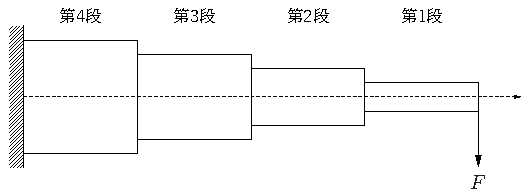
\includegraphics[width=.70\textwidth]{figures/ch04-06.pdf}
\caption*{图4.6\quad 由4段组成的悬臂梁。每段长度为一，截面为矩形。在梁的右端施加竖直力 $F$。}
\end{figure}
设计变量是 $N$ 段的宽度 $w_i$ 和高度 $h_i$。目标是在若干设计约束下最小化梁的总体积，它与重量成正比：
\[
w_1h_1+\cdots+w_Nh_N.
\]
对各段宽度和高度施加上下界
\[
w_{\min}\le w_i\le w_{\max},\quad h_{\min}\le h_i\le h_{\max},\quad i=1,\ldots,N,
\]
并对高宽比施加约束
\[
S_{\min}\le h_i/w_i\le S_{\max}.
\]
此外，对材料最大允许应力和梁端竖直挠度施加限制。

先考虑最大应力约束。第 $i$ 段的最大应力记为 $\sigma_i$，由 $\sigma_i=6iF/(w_ih_i^2)$ 给出。施加约束
\[
\frac{6iF}{w_ih_i^2}\le\sigma_{\max},\quad i=1,\ldots,N,
\]
即可保证梁内任何位置的应力都不超过最大允许值 $\sigma_{\max}$。

最后一个约束限制梁端竖直挠度，记梁端挠度为 $y_1$：
\[
y_1\le y_{\max}.
\]
挠度 $y_1$ 可由涉及各段挠度和斜率的递推求得：
\begin{equation}
\begin{aligned}
v_i&=12(i-1/2)\frac{F}{Ew_ih_i^3}+v_{i+1},\\
y_i&=6(i-1/3)\frac{F}{Ew_ih_i^3}+v_{i+1}+y_{i+1},
\end{aligned}\tag{4.45}
\end{equation}
其中 $i=N,N-1,\ldots,1$，初始值为 $v_{N+1}=y_{N+1}=0$。递推中，$y_i$ 为第 $i$ 段右端的挠度，$v_i$ 为该处斜率。利用（4.45）可以证明，这些挠度和斜率实际上都是变量 $w,h$ 的正项式函数。

% Source PDF page 179 (printed p. 165)
先注意 $v_{N+1}$ 和 $y_{N+1}$ 均为零，因此是正项式。假设 $v_{i+1},y_{i+1}$ 是 $w,h$ 的正项式函数。（4.45）的左式说明，$v_i$ 是一个单项式和正项式 $v_{i+1}$ 之和，因而为正项式。由右式可知，挠度 $y_i$ 是一个单项式及两个正项式 $v_{i+1},y_{i+1}$ 之和，所以也是正项式。特别地，梁端挠度 $y_1$ 是正项式。

于是问题为
\begin{equation}
\begin{array}{ll}
\text{最小化}&\displaystyle\sum_{i=1}^N w_ih_i\\
\text{约束为}&w_{\min}\le w_i\le w_{\max},\quad i=1,\ldots,N,\\
&h_{\min}\le h_i\le h_{\max},\quad i=1,\ldots,N,\\
&S_{\min}\le h_i/w_i\le S_{\max},\quad i=1,\ldots,N,\\
&6iF/(w_ih_i^2)\le\sigma_{\max},\quad i=1,\ldots,N,\\
&y_1\le y_{\max},
\end{array}\tag{4.46}
\end{equation}
变量为 $w,h$。这是GP，因为目标为正项式，全部约束均能写成正项式不等式。（实际上，除挠度上限是复杂的正项式不等式之外，其余约束均可写成单项式不等式。）

分段数 $N$ 很大时，正项式 $y_1$ 中的单项式项数大致按 $N^2$ 增长。习题4.31将研究另一种表述：引入变量 $v_1,\ldots,v_N,y_1,\ldots,y_N$，并用修改后的递推关系作为一组约束。这种表述避免了单项式项数的增长。

\subsubsection*{利用Perron--Frobenius理论最小化谱半径}
设矩阵 $A\in\R^{n\times n}$ 逐元素非负，即 $A_{ij}\ge0$（$i,j=1,\ldots,n$），并且不可约，即矩阵 $(I+A)^{n-1}$ 逐元素为正。Perron--Frobenius定理指出，$A$ 有一个正实特征值 $\lambda_{\mathrm{pf}}$，等于其谱半径，即全部特征值模的最大值。Perron--Frobenius特征值 $\lambda_{\mathrm{pf}}$ 决定 $k\to\infty$ 时 $A^k$ 的渐近增长或衰减速度；事实上，矩阵 $((1/\lambda_{\mathrm{pf}})A)^k$ 收敛。粗略地说，$k\to\infty$ 时，若 $\lambda_{\mathrm{pf}}>1$，$A^k$ 按 $\lambda_{\mathrm{pf}}^k$ 增长；若 $\lambda_{\mathrm{pf}}<1$，则按 $\lambda_{\mathrm{pf}}^k$ 衰减。

非负矩阵理论的一项基本结果为
\[
\lambda_{\mathrm{pf}}=\inf\{\lambda\mid\text{存在 }v\succ0\text{，使 }Av\preceq\lambda v\},
\]
而且下确界能够达到。不等式 $Av\preceq\lambda v$ 可以表示为
\begin{equation}
\sum_{j=1}^n\frac{A_{ij}v_j}{\lambda v_i}\le1,\quad i=1,\ldots,n,\tag{4.47}
\end{equation}
这是一组关于变量 $A_{ij},v_i,\lambda$ 的正项式不等式。因此，条件 $\lambda_{\mathrm{pf}}\le\lambda$ 可表示为关于 $A,v,\lambda$ 的一组正项式不等式。这使得一些涉及Perron--Frobenius特征值的优化问题可以用几何规划求解。

% Source PDF page 180 (printed p. 166)
假设矩阵 $A$ 的元素是某个底层变量 $x\in\R^k$ 的正项式函数。此时不等式（4.47）是关于变量 $x\in\R^k,v\in\R^n,\lambda\in\R$ 的正项式不等式。考虑选择 $x$ 以最小化 $A$ 的Perron--Frobenius特征值或谱半径，并可对 $x$ 施加正项式不等式约束：
\[
\begin{array}{ll}\text{最小化}&\lambda_{\mathrm{pf}}(A(x))\\\text{约束为}&f_i(x)\le1,\quad i=1,\ldots,p,\end{array}
\]
其中 $f_i$ 为正项式。利用上述刻画，可将问题表示为GP
\[
\begin{array}{ll}\text{最小化}&\lambda\\\text{约束为}&\displaystyle\sum_{j=1}^n A_{ij}v_j/(\lambda v_i)\le1,\quad i=1,\ldots,n,\\&f_i(x)\le1,\quad i=1,\ldots,p,\end{array}
\]
变量为 $x,v,\lambda$。

作为具体例子，考虑一种细菌种群动态的简单模型，以 $t=0,1,2,\ldots$ 表示时间或时期，单位为小时。向量 $p(t)\in\R_+^4$ 描述第 $t$ 期的种群年龄分布：$p_1(t)$ 为年龄在0至1小时之间的细菌总数，$p_2(t)$ 为年龄在1至2小时之间的细菌总数，其余类推。我们任意假设细菌寿命不超过4小时。种群随时间按 $p(t+1)=Ap(t)$ 演化，其中
\[
A=\begin{bmatrix}b_1&b_2&b_3&b_4\\s_1&0&0&0\\0&s_2&0&0\\0&0&s_3&0\end{bmatrix}.
\]
这里 $b_i$ 为第 $i$ 年龄组的繁殖率，$s_i$ 为由第 $i$ 年龄组存活至第 $i+1$ 年龄组的比例。假设 $b_i>0$、$0<s_i<1$，从而矩阵 $A$ 不可约。

$A$ 的Perron--Frobenius特征值决定种群的渐近增长或衰减速度。若 $\lambda_{\mathrm{pf}}<1$，种群按 $\lambda_{\mathrm{pf}}^t$ 衰减至零，因此半衰期为 $-1/\log_2\lambda_{\mathrm{pf}}$ 小时。若 $\lambda_{\mathrm{pf}}>1$，种群按 $\lambda_{\mathrm{pf}}^t$ 几何增长，倍增时间为 $1/\log_2\lambda_{\mathrm{pf}}$ 小时。最小化 $A$ 的谱半径，对应寻找种群最快的衰减速度或最慢的增长速度。

作为矩阵 $A$ 所依赖的底层变量，取环境中影响细菌繁殖率和存活率的两种化学物质浓度 $c_1,c_2$。将繁殖率和存活率建模为两种浓度的单项式函数：
\[
\begin{aligned}
b_i&=b_i^{\mathrm{nom}}(c_1/c_1^{\mathrm{nom}})^{\alpha_i}(c_2/c_2^{\mathrm{nom}})^{\beta_i},\quad i=1,\ldots,4,\\
s_i&=s_i^{\mathrm{nom}}(c_1/c_1^{\mathrm{nom}})^{\gamma_i}(c_2/c_2^{\mathrm{nom}})^{\delta_i},\quad i=1,\ldots,3.
\end{aligned}
\]
这里 $b_i^{\mathrm{nom}}$ 为标称繁殖率，$s_i^{\mathrm{nom}}$ 为标称存活率，$c_i^{\mathrm{nom}}$ 为第 $i$ 种化学物质的标称浓度。常数 $\alpha_i,\beta_i,\gamma_i,\delta_i$ 给出化学物质浓度偏离标称值时对繁殖率和存活率的影响。
